\documentclass[12pt,a4paper]{article}
\usepackage[UTF8]{ctex}
\usepackage{graphicx}
\usepackage{geometry}
\usepackage{ulem}
\usepackage{enumitem}
\usepackage{titlesec}
\usepackage{multicol}
\usepackage[export]{adjustbox}
\usepackage{amsmath}  % 推荐用于更好的数学排版
\usepackage[utf8]{inputenc}
\usepackage{CJKutf8}
\usepackage{fancyhdr}
\usepackage{lastpage}
\usepackage{ulem}
\usepackage{tabularx}
\usepackage{lastpage}
\usepackage{float}
% 页眉页脚设置
\pagestyle{fancy}
\fancyhf{} % 清除所有页眉页脚
% 设置页眉内容
%-==========1. 填写从第二页开始 每页第一行的信息==========-
\fancyhead[C]{
    \makebox[4.5em][c]{实验名称：} \uline{\makebox[14em][c]{集成运算放大器应用电路研究(II)}} 
    \makebox[2.5em][c]{姓名：} \uline{\makebox[4em][c]{}} 
    \makebox[2.5em][c]{学号：} \uline{\makebox[5em][c]{}}
}%--------------------------------------------------------
\fancyfoot[C]{第 \thepage\ 页，共 \pageref{LastPage} 页}

% 取消页眉和页脚的下划线
\renewcommand{\headrulewidth}{0pt} % 页眉横线粗细设为0
\renewcommand{\footrulewidth}{0pt} % 页脚横线粗细设为0

% 调整页眉高度
\setlength{\headheight}{50pt}

% 设置plain样式（用于第一页）
\fancypagestyle{plain}{
    \fancyhf{} % 清除所有页眉页脚
    \renewcommand{\headrulewidth}{0pt} % 隐藏页眉横线
    \fancyfoot[C]{第 \thepage\ 页，共 \pageref{LastPage} 页} % 保留页脚
}
% 设置页面边距
\geometry{left=2.54cm,right=1.5cm,top=2.54cm,bottom=2.54cm}

% 设置正文字体大小为小四
\renewcommand{\normalsize}{\fontsize{12pt}{18pt}\selectfont}
% 设置章节格式
\titleformat{\section}{\fontsize{16pt}{24pt}\selectfont\bfseries}{\thesection}{1em}{} % 一级标题：三号
\titleformat{\subsection}{\fontsize{15pt}{22.5pt}\selectfont\bfseries}{\thesubsection}{1em}{} % 二级标题：小三

\begin{document}
\thispagestyle{plain}%第一页使用 plain 样式，而不是默认的 fancy 样式，第一页不再显示页眉
% 标题部分 - 两栏布局
\begin{multicols}{2}
    % 左栏：图片和实验报告标题
    % 左栏：使用空行创建前三行
    \noindent
    ~\\ % 第一行
    ~\\ % 第二行
    ~\\ % 第三行
    \hphantom{占位}% 使用空占位符
    \raisebox{-0.5\baselineskip}% 图片向下移动半行
    {
\includegraphics[width=1.85in,height=0.58in]{figure/ZJU.jpg}}
    \hspace{.5em}% 图片和标题之间的间距
    \raisebox{0pt}[\height][0pt]% 标题底部对齐
    {\textbf{\fontsize{26pt}{30pt}\selectfont 实验报告}}
    
    \columnbreak % 换到右栏
    
    % 右栏：个人信息
    % 右栏：个人信息 - 靠右对齐 
%-==========2. 填写个人信息==========-
    \begin{flushright}
        \makebox[3em][l]{专业：} \uline{\makebox[9em][c]{}} \\
        \makebox[3em][l]{姓名：} \uline{\makebox[9em][c]{}} \\
        \makebox[3em][l]{学号：} \uline{\makebox[9em][c]{}} \\
        \makebox[3em][l]{日期：} \uline{\makebox[9em][c]{2025年12月23日}} \\
        \makebox[3em][l]{地点：} \uline{\makebox[9em][c]{紫金港东四216}} \\
    \end{flushright}   
\end{multicols}
% 课程名称等信息（单栏）
%-==========3. 填写课程信息==========-
\noindent\small
课程名称： \uline{电子电路设计实验I} \hfill 指导老师： \uline{施红军、叶险峰、邓靖靖} \hfill 成绩： \uline{\hspace{3cm}} \\
实验名称： \uline{集成运算放大器应用电路研究(II)} \hfill 实验类型： \uline{设计类实验} \hfill 同组学生姓名： \uline{}
%-==========4. 正文开始==========-
\section*{一、实验目的}

1.学习和研究由集成运放构成的积分器、比较
器、波形发生器等应用电路的组成与原理，
掌握其设计方法。

2.观察积分运算电路在实际应用时存在的积分
漂移、积分误差等现象，了解解决方法。
\section*{二、实验任务与要求}
1.设计并搭建由集成运放构成的积分器。

2.设计搭建迟滞比较器电路。

3.设计并搭建方波/三角波发生器电路。

\section*{三、实验原理}
(1) \textbf{反相积分器}

积分器将反相比例放大器的反馈电阻 \(R_2\) 替换为电容 \(C\)。其输出电压是输入电压对时间的积分，即 \(v_o(t) = -\frac{1}{R_1C} \int v_i(t) dt + u_O(0)\)。常用于波形变换（如方波变三角波）、模数转换及控制系统等。

电路图如下：
\begin{figure}[H]
    \centering
    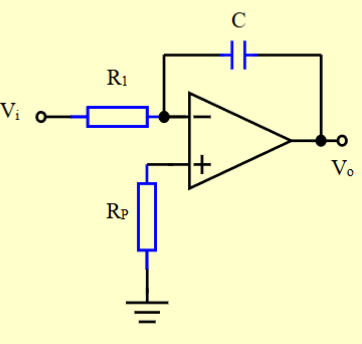
\includegraphics[width=0.4\textwidth]{figure/circuit_in.png}
    \caption{积分器电路图}
\end{figure}

当输入信号为阶跃信号时，理想积分器的输出为斜坡信号。
\[V_i(t)=Eu(t)
\]
\[V_o(t)=-\frac{E}{R_1C}t
\]

因此可以得到方波信号积分为三角波信号。且振幅为 \(E\)，周期为 \(T\) 的方波信号经过积分器后输出的三角波信号振幅为 \(V_{om}=\frac{ET}{4R_1C}\)。

但由于输入信号的直流分量、输入失调电压的存在，实际电路中积分器的输出会出现积分漂移现象。为减小漂移，可在反馈回路中并联一个大阻值电阻 \(R_f\)，使电路在低频时表现为反相比例放大器，从而限制输出电压的漂移。

同时由于引入了反馈电阻 \(R_f\)，使得电路在高频时不再是理想积分器，积分特性受到影响。因此应尽量选择较大的 \(R_f\) 以减小对积分特性的影响。

一般取 \(R_f > 10 R_1\)。

(2) \textbf{迟滞比较器}

迟滞比较器是一种具有滞回特性的比较器，其输出电压在输入电压超过某一上限阈值时跳变为高电平，在输入电压低于某一下限阈值时跳变为低电平。这样可以有效抑制输入信号中的噪声干扰，防止输出频繁跳变。

电路图如下：
\begin{figure}[H]
    \centering
    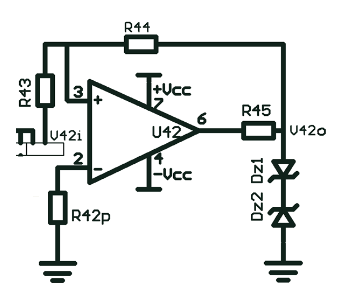
\includegraphics[width=0.4\textwidth]{figure/circuit_compare.png}
    \caption{迟滞比较器电路图}
\end{figure}
运放正相位端口电压满足
\[V_+=\frac{R_{43}}{R_{43}+R_{44}}v_{42o}+\frac{R_{44}}{R_{43}+R_{44}}V_{42i}
\]
运算放大器的输出端口为高电平时有
\[v_{42o}=V_Z+V_D
\]
$V_{42i} > - \frac{R_{43}}{R_{44}}(V_Z+V_D)$时输出稳定为高电平。
$V_{42i} < - \frac{R_{43}}{R_{44}}(V_Z+V_D)$时输出翻转为低电平。

记$$V_{TH}=- \frac{R_{43}}{R_{44}}(V_Z+V_D)$$
为阈值电压。

运算放大器的输出端口为低电平时有
\[v_{42o}=-(V_Z+V_D)
\]
$V_{42i} < V_{TH}=\frac{R_{43}}{R_{44}}(V_Z+V_D)$时输出稳定为低电平。
$V_{42i} > V_{TH}=\frac{R_{43}}{R_{44}}(V_Z+V_D)$时输出翻转为高电平。

传输特性曲线如下：
\begin{figure}[H]
    \centering
    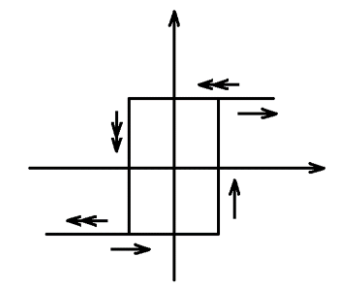
\includegraphics[width=0.4\textwidth]{figure/transfer_hysteresis.png}
    \caption{迟滞比较器传输特性曲线}
\end{figure}

输入输出波形如下：
\begin{figure}[H]
    \centering
    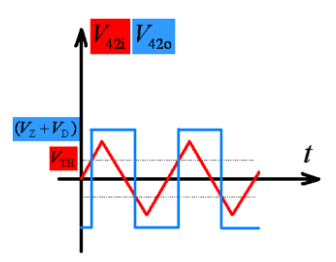
\includegraphics[width=0.4\textwidth]{figure/waveform_hysteresis.png}
    \caption{迟滞比较器输入输出波形}
\end{figure}

(3) \textbf{方波、三角波发生器}

方波、三角波发生器由积分器和迟滞比较器组成。迟滞比较器输出方波信号，积分器将方波信号积分为三角波信号。通过调节电路参数，可以控制输出波形的频率和幅度。

\section*{四、实验方案设计与参数计算}

(1) 积分器设计

输入信号方波要求幅度2.2V，频率500Hz，输出信号为幅度2V左右的三角波。电容值为22nF.

根据积分器输出幅度公式
\[V_{om}=\frac{ET}{4R_1C}
\]
则有
\[R_1=\frac{ET}{4V_{om}C}=\frac{2.2\times \frac{1}{500}}{4\times 2 \times 22\times 10^{-9}}=25k\Omega
\]
实际选择标准阻值$R_1=24k\Omega$。

反馈电阻$R_f=270k\Omega$, 满足$R_f > 10 R_1$。

(2) 迟滞比较器设计

考虑设计一迟滞比较器，使$V_{TH} \approx \frac{1}{2}(V_Z+V_D)$
允许使用电阻值在20kΩ~400kΩ之间。安装电路，输入500Hz三角波（幅度合理自定），
研究输入、输出信号的幅度、相位关系。

根据阈值电压公式
\[V_{TH}=- \frac{R_{43}}{R_{44}}(V_Z+V_D)
\]
取$R_{44}=300k\Omega$，则$R_{43}=150k\Omega$, 三角波频率500Hz，幅度4V。

(3) 方波、三角波发生器设计

断开迟滞比较器信号输入，搭建方波-三角波发生电路，
调节电位器$R_{w4}$，可产生不同频率方波、三角波。
观察电压$V_{42o}'$与输出信号频率的关系，测量并记
录可调频率范围。


\section*{五、实验仪器设备}
信号发生器，电源，示波器，电路板等电子器件。

\section*{六、实验步骤、调试过程、实验数据记录}
(1) 积分器实验步骤与数据记录

选取电阻$R_{1}=24k\Omega$，反馈电阻$R_{f}=270k\Omega$，电容$C=22 nF$，搭建积分器电路。

输入方波信号，频率500Hz，幅度2.2V，观察输入输出波形如下：
\begin{figure}[H]
    \centering
    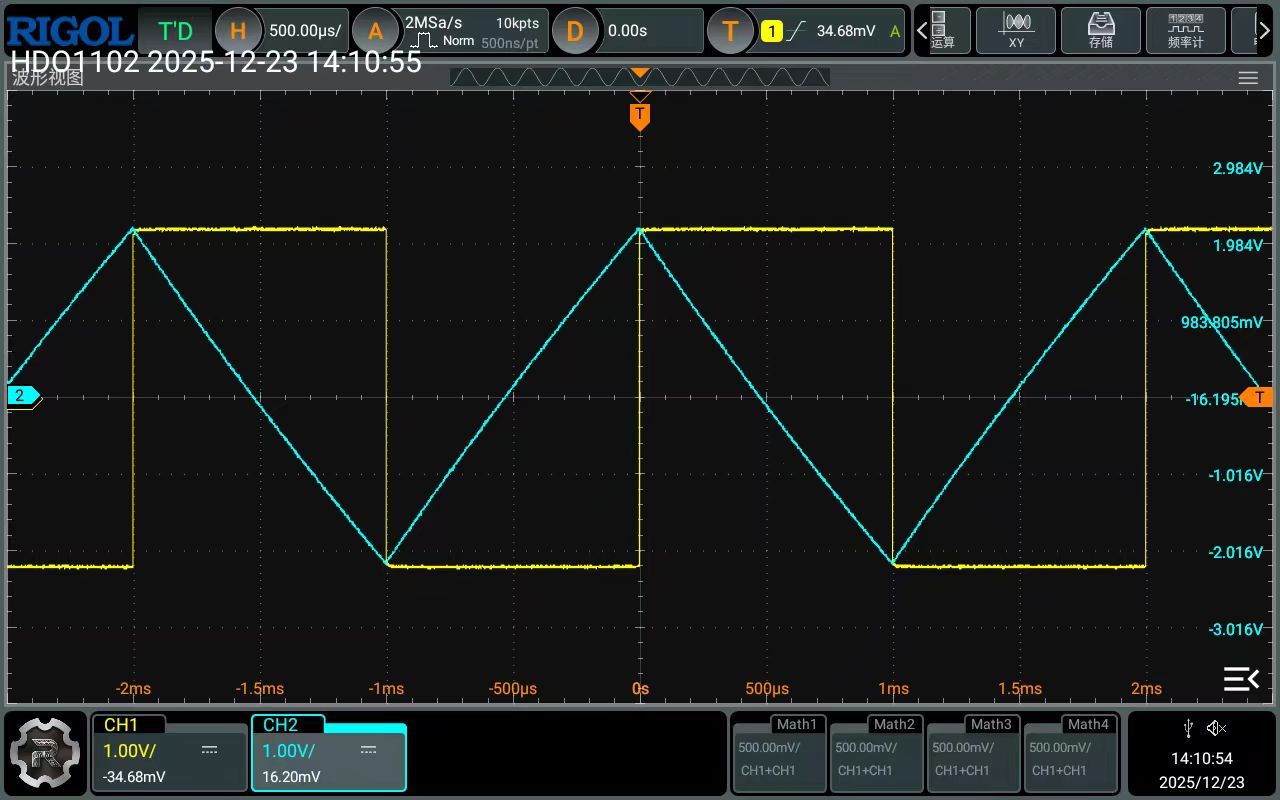
\includegraphics[width=0.4\textwidth]{figure/waveform_integrator.jpg}
    \caption{积分器输入输出波形}
\end{figure}

测量得到输出三角波峰峰值$V_{o}=4.4217V$，直流分量为1.437V。输入方波峰峰值$V_{41i}=4.4565V$。

(2) 迟滞比较器实验步骤与数据记录

选择电阻$R_{43}=150k\Omega$，$R_{44}=300k\Omega$，搭建迟滞比较器电路。
输入500Hz三角波，幅度4V，观察输入输出波形如下注，可以看到输入信号于输出信号相位有明显差异。
\begin{figure}[H]
    \centering
    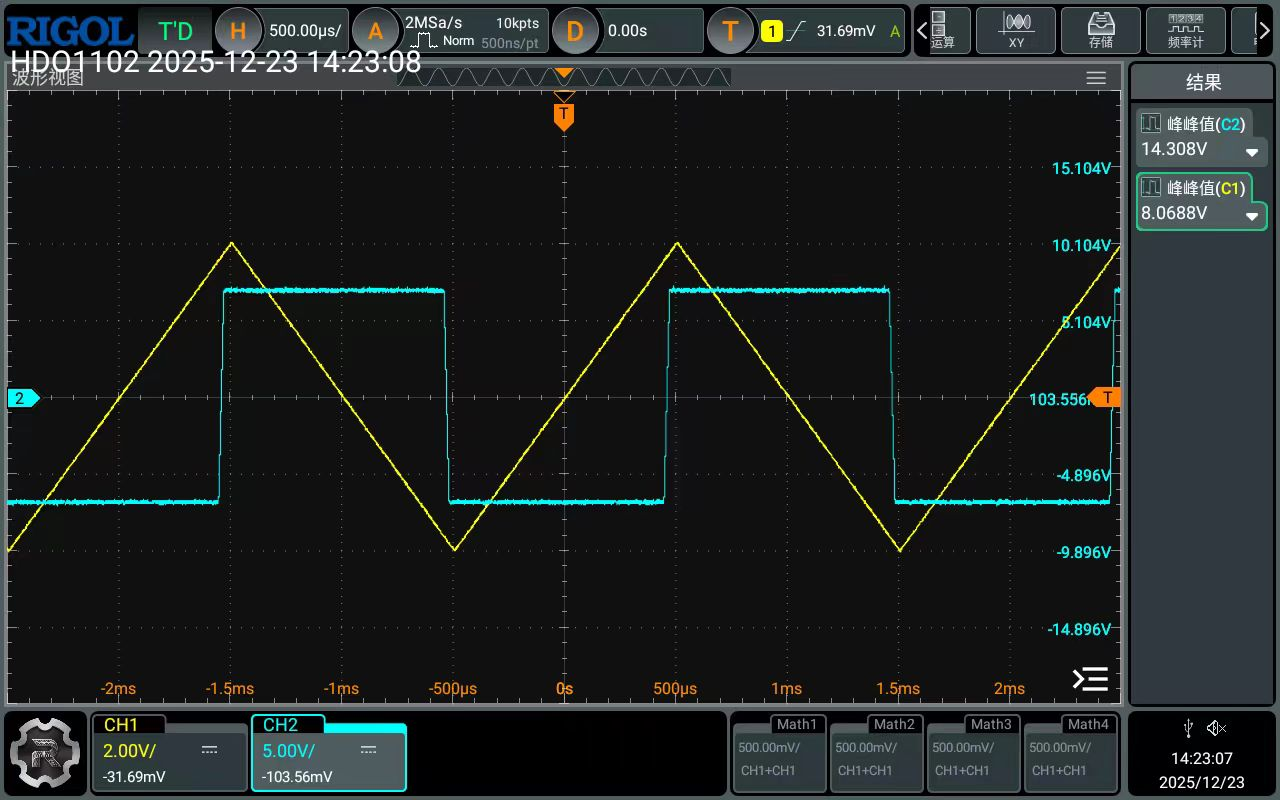
\includegraphics[width=0.4\textwidth]{figure/waveform_hysteresis_exp.jpg}
    \caption{迟滞比较器输入输出波形}
\end{figure}

测量得到阈值电压$V_{TH}=3.562V$，与理论值(3.5V左右)符合较好。

输出方波峰峰值$V_{42o}=14.308V$,与预期的$2(V_Z+V_D) \approx 13.8V$比较接近。输入三角波峰峰值$V_{42i}=8.0645V$。

(3) 方波、三角波发生器实验步骤与数据记录

调节电位器$R_{w4}$，观察输出波形频率变化情况.
\begin{figure}[H]
    \centering
    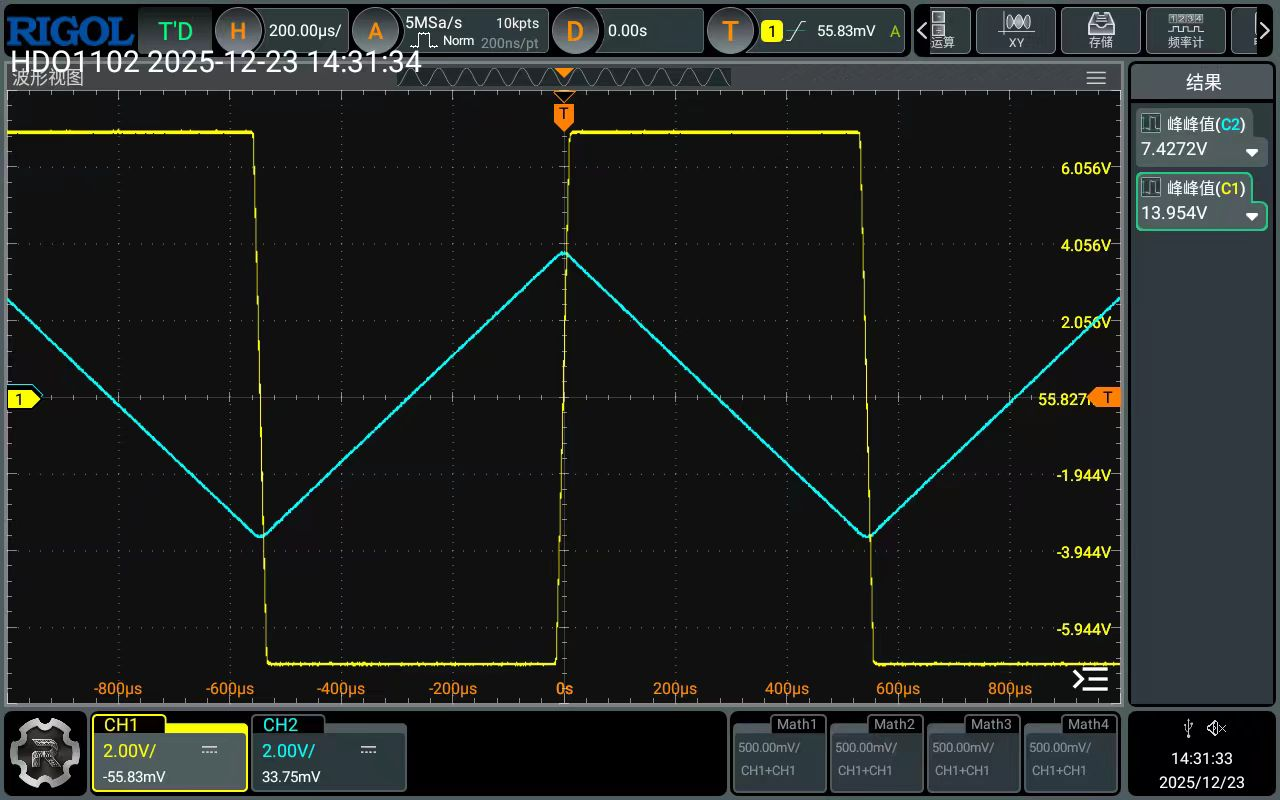
\includegraphics[width=0.4\textwidth]{figure/waveform_wavegen.jpg}
    \caption{方波、三角波发生器输出波形}
\end{figure}
发现当顺时针转到电位器时，电压$V_{42o}'$变小，输出信号频率变小，最小可至0Hz

反之亦然，逆时针转到电位器时电压$V_{42o}'$变大，输出信号频率变大，频率最大值为917.93Hz。
\section*{七、数据分析与讨论}

1. \textbf{积分器实验分析}

根据实验数据，输入方波峰峰值 $V_{41i}=4.4565\mathrm{V}$（幅度 $E=2.228\mathrm{V}$），输出三角波峰峰值 $V_o=4.4217\mathrm{V}$（幅度 $V_{om}=2.211\mathrm{V}$）。代入积分器输出幅度公式进行验证：
\[
V_{om} = \frac{ET}{4R_1C} = \frac{2.228 \times \frac{1}{500}}{4 \times 24\times 10^3 \times 22\times 10^{-9}} \approx 2.108\mathrm{V}
\]
理论计算值（$2.108\mathrm{V}$）与实测值（$2.211\mathrm{V}$）相对误差约为 $4.9\%$。误差主要来源于电阻电容的实际值与标称值存在偏差，以及示波器测量时的读数误差。

输出波形存在 $1.437\mathrm{V}$ 的直流分量，这主要是由运放的输入失调电压、输入偏置电流以及积分电容的漏电流等因素引起的积分漂移现象。并联的反馈电阻 $R_f=270\mathrm{k\Omega}$（满足 $R_f > 10R_1$）在一定程度上限制了低频增益，抑制了漂移的无限增长，但引入 $R_f$ 也使得电路在低频段偏离理想积分特性。

2. \textbf{迟滞比较器实验分析}

实测阈值电压 $V_{TH}=3.562\mathrm{V}$。
稳压管稳压值 $V_Z \approx 6.2\mathrm{V}$，二极管正向压降 $V_D \approx 0.7\mathrm{V}$，因此 $V_Z+V_D \approx 6.9\mathrm{V}$。理论阈值电压为：
\[
V_{TH} = \frac{R_{43}}{R_{44}}(V_Z+V_D) = \frac{150}{300} \times 6.9 \approx 3.45\mathrm{V}
\]
实测值与理论值相对误差约为 $3.2\%$，吻合较好。误差来源于电阻精度、稳压管实际稳压值及二极管压降与典型值的偏差。

输出方波峰峰值实测为 $14.308\mathrm{V}$，理论值应为 $2(V_Z+V_D) \approx 13.8\mathrm{V}$，误差约为 $3.7\%$。迟滞比较器有效避免了输入三角波在阈值电压附近因噪声可能引起的输出抖动，展示了其良好的抗干扰能力。

3. \textbf{方波/三角波发生器实验分析}

发生器由迟滞比较器与积分器构成正反馈环路。调节电位器 $R_{w4}$ 改变了积分器的充电电流，从而改变了积分斜率，最终调节了输出波形的频率。实验测得频率调节范围为 $0\mathrm{Hz}$（接近直流）至 $917.93\mathrm{Hz}$，实现了宽范围频率可调。

对比单独积分器实验，此时三角波幅度由电路内部参数（比较器输出幅度、积分电阻电容）自动设定，而非由外部输入信号决定，电路实现了自激振荡。
\section*{八、结论}

1. 成功设计并搭建了反相积分器电路，实现了方波到三角波的线性变换。实验验证了积分器输出幅度公式，并观测到了积分漂移现象，通过并联大阻值反馈电阻 $R_f$ 对其进行了有效抑制。

2. 成功设计并搭建了迟滞比较器电路，其传输特性与理论分析一致，实测阈值电压与理论值误差仅为 $3.2\%$，验证了其能有效克服噪声干扰，避免输出在临界点附近的反复跳变。

3. 成功将积分器与迟滞比较器级联，构成了方波/三角波发生器。电路通过调节单个电位器即可实现输出频率从 $0\mathrm{Hz}$ 到 $917.93\mathrm{Hz}$ 的连续可调，波形稳定，达到了设计要求。

本实验验证了集成运放在波形变换、信号比较和波形产生方面的基本应用，深化了对积分器、比较器及其构成振荡电路工作原理的理解。

\section*{九、心得与体会}

通过本次实验，我对集成运放的应用有了从理论到实践的深入认识。积分器部分让我直观体会到理想元件与实际器件的差异，特别是积分漂移现象，理解了在反馈回路中并联电阻进行补偿的工程方法。迟滞比较器实验让我认识到引入正反馈可以塑造电路的“记忆”特性，提高抗干扰能力的实际意义。最后，将两个单元电路组合成波形发生器的过程，让我深刻体会到模拟电路系统级设计的思路：通过功能模块的有机连接，可以实现更复杂的信号处理功能。

在调试过程中，我也遇到了一些挑战，如积分器输出直流偏移过大、波形发生器不起振等。通过检查电路连接、测量关键点电压、逐步调整参数，最终解决了问题。这个过程锻炼了我的电路调试能力和耐心。此外，示波器的熟练使用和实验数据的准确记录与分析，也是本次实验的重要收获。理论计算与实测结果之间的误差分析，促使我思考元器件公差、测量误差等因素的影响，这对培养严谨的工程思维至关重要。
\section*{十、思考题}
1. 反相输入滞回比较器与同相输入滞回比较器的传输特性曲线有何不同？

答：两者的传输特性曲线形状相似，均为滞回曲线，但方向不同。
对于反相输入滞回比较器，当输入电压 $v_i$ 逐渐增大时，输出电压 $v_o$ 在 $v_i$ 
达到上门限电压 $V_{T+}$ 时从高电平跳变为低电平；
当 $v_i$ 逐渐减小时，$v_o$ 在 $v_i$ 降至下门限电压 $V_{T-}$ 时从低电平跳回高电平。
其跳变方向是“向上增，向下跳；向下减，向上跳”。
而同相输入滞回比较器的跳变方向正好相反，是“向上增，向上跳；向下减，向下跳”。
即两者的滞回曲线关于原点对称（假设高低电平对称）。

2.为什么说过零比较器的抗干扰能力差，怎样改进提高比较器抗干扰能力？

答：过零比较器只有一个阈值电压（$0\mathrm{V}$）。
当输入信号在零点附近存在微小噪声或干扰时，会导致输出电压在高低电平之间频繁、错误地跳变，
无法得到稳定的输出。
改进方法是引入正反馈，构成迟滞比较器（滞回比较器）。
这样电路就有两个不同的阈值电压（上门限 $V_{T+}$ 和下门限 $V_{T-}$）。
输入信号必须超过 $V_{T+}$ 才能令输出从高变低，必须低于 $V_{T-}$ 才能令输出从低变高。
两个阈值之间的电压差（回差电压）形成了一个“死区”，
只要干扰信号的幅度小于回差电压，就不会引起输出的误动作，从而显著提高了抗干扰能力。

3.如何用运放产生锯齿波？

答：产生锯齿波的核心思想是让电容进行慢充电和快放电（或反之），形成上升斜率与下降斜率显著不同的三角波，即为锯齿波。常用方法有以下两种：

(1) \textbf{利用积分器和电子开关}：在方波-三角波发生器的基础上，在积分电容的充电回路和放电回路中设置不同的电阻（或电流源）。例如，用一个电阻和一个二极管并联，使电容充电时经过电阻，放电时经过二极管（导通电阻小），即可得到上升慢（或快）、下降快（或慢）的锯齿波。

(2) \textbf{利用恒流源对电容充放电}：用运放和晶体管构成恒流源，对电容进行恒流充电，产生线性斜坡电压（三角波的半边）。当电压达到比较器的阈值时，控制电路使恒流源反向或使电容快速放电/复位，然后开始下一个周期的充电，从而产生锯齿波。这种方法线性度更好。

\end{document}